%
% Layout retirado de http://www.di.uminho.pt/~prh/ii02pd.html
%
%\documentclass[twocolumns]{article}
\documentclass{article}

\usepackage[portuges]{babel}
\usepackage[utf8]{inputenc}
\usepackage{csquotes}
\usepackage{hyperref}
\hypersetup{
    colorlinks,
    citecolor=black,
    filecolor=black,
    linkcolor=black,
    urlcolor=black
}

\usepackage{graphicx}
\usepackage{float}

\parindent=0pt
\parskip=2pt


\title{Processamento de Linguagens - TP2 - Processador para LaTex}
\author{Gonçalo Camaz \\ A76861
        \and
        Jorge Oliveira\\ A78660
        \and José Ferreira\\ A78452 }
\date{ (\today)}

\begin{figure}
  \centering
  
\includegraphics[width=0.5\linewidth]{1.jpg}
\end{figure}

\begin{document}

\maketitle

\pagebreak

\begin{abstract}
No presente relatório vamos apresentar uma linguegem mais leve do que o latex e o programa que trasformar a mesma em texto latex.
Apresentamos a nossa linguagem e as suas caraterísticas, a forma de colocar o texto com ênfase(negrito, itálico e sublinhado) e também de listas, tabelas e vários níveis de "cabeçalhos".
Depois apresentamos também como realizamos o processo de transformação da nossa linguagem para latex com o auxílio da ferramenta \textit{Flex} e das suas caraterísticas bastante poderosas, nomeadamente as condições de contexto.
\end{abstract}

\tableofcontents

\listoffigures

\pagebreak

\section{Introdução}

O presente relatório serve para descrever todo o processo para a criação de uma linguagem, que tem como objetivo facilitar a escrita de texto com a sintaxe do \LaTeX.

O nosso principal objetivo era conseguir realizar todos os desafios propostos no enunciado. Só após esta base estar pronta é que pensaríamos em realizar algo mais, que poderia passar, pela abstração de tabelas ou então o encadeamento de marcas.

Tal tarefa deve ser efetuada usando o \textit{flex}. Este é também um outro objetivo, tentar usar ao máximo o \textit{flex} e não cair no erro de tentar resolver o problema usando código C.



\section{Estrutura do Relatório} 
No capítulo~\ref{ae} será feita uma apresentação do problema que estamos a tratar e ainda a linguagem que nós construímos. Desta forma o leitor terá um melhor enquadramento sobre o porquê de realizarmos este trabalho e ainda a constituição da linguagem. \par

No capítulo~\ref{cdr} apresentaremos a forma como abordamos o problema em termos algorítmicos e no capítulo~\ref{ct} serão apresentados os resultados obtidos pelo nosso programa. O capítulo~\ref{concl} concluí o relatório com a apresentação da conclusão.



\section{Análise e Especificação} \label{ae}
\subsection{Descrição informal do problema}

O latex é bastante utilizado pela comunidade científica e matemática mundial devido à sua grande qualidade tipográfica. O LaTeX fornece um conjunto de macros alto-nível que tornam mais fácil e rápida a produção de documentos em TeX e é utilizado para produzir todo o tipo de documentos. \par

O principal objetivo do LaTeX é que o autor se possa distanciar da apresentação visual do documento e assim concentrar-se no seu conteúdo. Possui variadíssimas formas de lidar com bibliografias, citações, formatos de páginas, referências e tudo mais que não seja relacionado com conteúdo do documento em si. \par

Porém, é necessário, editar o próprio texto para colocar com a sintaxe do LaTeX, um ato que por vezes se torna maçador. O ideal seria termos um conjunto de anotações mais simples e mais intuitivas na sua escrita (o ideal seria até que estas anotações fossem o máximo independente da escrita em LaTeX), e que depois de executar um pré-processamento estas anotações mais simples se transformassem em anotações de acordo com o LaTeX. Um caso deste é o \textit{MarkDown}. \par

O nosso objetivo, com a conceção deste trabalho, é criar umas anotações mais simples para a escrita de documentos em LaTeX. De modo que, quem esteja a escrever o seu texto, se foque essencialmente no texto e se abstraia mais de qual comando tem de colocar para que o seu texto fique editado de uma forma correta.

\subsection{Apresentação da Linguagem}


Como já foi referido anteriormente, o LaTeX tem uma vasta biblioteca para a edição correta do texto, mas nós focámo-nos nos marcadores que possam ser mais utilizados. A escrita em negrito, itálico ou sublinhado e ainda vários níveis de títulos (\textit{chapter, section, subsection, subsubsection}). Vários tipos de lista, numeradas, não-numeradas e dicionário. E ainda o uso de tabelas.

De seguida passamos a apresentar a linguagem utilizada:

O símbolo \$ indica o nível da \textit{section}. Um \$ indica que é uma \textit{section}, \$\$ indica \textit{subsection} e \$\$\$ \textit{subsubsection}.

\*palavra\* -  Caso uma sequência de carateres esteja entre dois asteriscos então é uma indicação de que deve ser escrita em negrito. Para esta anotação, inspirámo-nos no que uma aplicação bem conhecida já faz. O Facebook, caso coloquemos algo entre dois asteriscos, automaticamente aplica um efeito de negrito.

\&palavra\& - Caso uma sequência de carateres esteja entre dois \& significa que essa sequência vai ser escrita em itálico. Para esta anotação, baseámo-nos na anterior, e para que fosse mais intuitivo colocamos o símbolo do \“E comercial\”.

\_palavra\_ - Caso uma sequência de carateres esteja entre dois \textit[underscores} significa que essa sequência vai ser sublinhada. Para esta anotação, baseámo-nos mais  uma vez nas anteriores, e utilizamos o ‘\_’ já que da a ideia de que a palavra deve ser sublinhada ao utilizador.

Tratamento das Listas:

Os seguintes símbolos indicam o inicio de uma lista. Para tal, o utilizador deve colocar a seguinte sintaxe: \#Opção\# sendo que a “Opção” deve ser um carater dentro do seguinte conjunto: \{O,N,D\}.

\#O\# - Inicio de uma lista do tipo ordenada.

\#N\# - Inicio de uma lista do tipo não ordenada.

\#D\# - Inicio de uma lista do tipo dicionário.

Após a indicação do inicio da lista, seguem-se os vários elementos, que devem ser escritos também eles entre os símbolos cardinais.

Quando terminar a escrita dos vários elementos, deverá colocar o seguinte símbolo \#FOpção\# (Opção pertence \{O,N,D\}), que deverá corresponder ao inicio da lista que o utilizador iniciou.

Tratamento da Tabela:
Para a escrita da tabela o utilizador deverá iniciar através do símbolo #F#. Porém as tabelas trazem muitas variantes para a sua formatação. O grupo decidiu focar-se em realizar uma tabela simples, onde permitimos que de uma forma intuitiva o utilizador decida se pretende centrar a tabela, que coloque uma legenda para a mesma e ainda os vários elementos da tabela. De salientar que o utilizador deverá colocar a sintaxe do \textit{\\begin{tabular}}, já que traz variadíssimas opções e dessa forma, deixámos à escolha do utilizador quais as formatações que deseja.

\#F\# - Inicio de uma tabela.

\textgreater C - Inica que a tabela deve ser centrada (opcional)

\textgreater L legenda \textgreater FL - Adiciona uma legenda à tabela.

\textbar \hspace{} - A barra serve para separar cada elemento por coluna. Para a mudança de linha deve indicar um \#.

\#FT\# - Fim da tabela.

\subsection{Concepção/desenho da Resolução} \label{cdr}

Passada a fase de especificação da linguagem, estávamos em condições de passar para a implementação da aplicação que transforma a mesma em linguagem \textit{LaTex}. 
A primeira definição que realizamos foi quais seriam as condições de contexto que necessitamos para desenvolver a conversão. Como tínhamos diferentes parâmetros de conversões decidimos ter as seguintes condições de contexto:
\begin{itemize}
      \item LISTA - esta condição de contexto corresponde a texto que se encontra num contexto de lista ordenada ou não-ordenada
      \item NEGRITO - corresponde a texto que se encontra num contexto de negrito
      \item ITALICO - corresponde a texto que se encontra num contexto de itálico
      \item SUBLINHADO - corresponde a texto que se encontra num contexto de sublinhado
      \item CABECALHO - corresponde a texto que se encontra num contexto de cabeçalho
      \item DICIONARIO - corresponde a texto que se encontra num contexto de lista do tipo dicionário
      \item TABELA - corresponde a texto que se encontra num contexto de tabela
\end{itemize}
Depois verificamos que necessitávamos de uma \textit{stack} de condições de contexto pelo facto de que estas condições se poderiam aninhar umas nas outras (em certos casos), pelo que ativamos a opção \textit{stack} que nos fornece essa funcionalidade.
Começando pelo carater de escape que utilizamos sempre que encontrávamos texto com esse caractere (em qualquer contexto) seguido de um dos carateres definidos como especiais da linguagem imprimimos o texto, pois estava \textit{escaped}.
\begin{verbatim}
<*>\\[*_&#$] {printf("%s",yytext);}
\end{verbatim}
Sempre que em qualquer contexto encontrássemos também as expressões definidas como de início de alguma parte especial de texto então iniciamos essa parte e introduzimos o contexto referente na \textit{stack} através da operção \textbf{yy\_push\_state}. Antes de introduzir o contexto temos de imprimir o texto correspondente em \textit{LaTex} para início da parte em questão.
Exemplo do texto negrito:
\begin{verbatim}
<*>\*   { 
        printf("\\textbf{");
        yy_push_state(NEGRITO);
 
        }
\end{verbatim}
Exemplo do dicionário:
\begin{verbatim}
<*>#D# {
        printf("\\begin{description}");
        yy_push_state(DICIONARIO);
}
\end{verbatim}
No entanto, em certos casos nem sempre se pode iniciar a parte correspondente, por exemplo as tabelas não podem ser iniciadas em nenhum contexto, apenas no inicial o que acontece também com os cabeçalhos. Daí nestes casos termos definido que apenas realizamos a operação quando este se encontra na condição inicial.
Exemplo do cabeçalho:
\begin{verbatim}
$+  {
    int tam = strlen(yytext);
    switch(tam){
        case 1: printf("\\chapter{"); break;
        case 2: printf("\\section{"); break;
        case 3: printf("\\subsection{"); break;
        default: printf("\\subsubsection{");
    }
    yy_push_state(CABECALHO);
}
\end{verbatim}
Exemplo da tabela:
\begin{verbatim}
#T# {
    printf("\\begin{table}");
    yy_push_state(TABELA);
}
\end{verbatim}
Quando estamos num contexto e aparece a expressão que representa o fim do mesmo decidimos imprimir o caractere que corresponde ao fim do mesmo em \textit{LaTex} e de seguida retiramos o contexto da \textit{stack} através da operação \textbf{yy\_pop\_state}.
Exemplo de negrito:
\begin{verbatim}
<NEGRITO>\* {
        printf("}");
        yy_pop_state();
    }
\end{verbatim}
Exemplo de dicionário:
\begin{verbatim}
<DICIONARIO>#FD#    {
    printf("\\end{description}");
    yy_pop_state();
}
\end{verbatim}
Exemplo da tabela:
\begin{verbatim}
<TABELA>#FT# { printf("\\end{table}"); yy_pop_state();}
\end{verbatim}
Quando estamos num contexto de lista e identificamos a expressão que nos diz que estamos na presença de um novo item então temos de imprimir a expressão correspondente em \textit{LaTex}: \begin{verbatim} \item. \end{verbatim}
\begin{verbatim}
<LISTA>#    {

        printf("\\item");
}
\end{verbatim}
Quando aparece a expressão do fim de lista ordenada ou não ordenada também temos de imprimir o texto correspondente. Neste caso temos também de sair do contexto atual realizando a operação \textbf{yy\_pop\_state}.
\begin{verbatim}
<LISTA>#FO# {
    printf("\\end{enumerate}");
    yy_pop_state();
}

<LISTA>#FN# {
    printf("\\end{itemize}");
    yy_pop_state();
}
\end{verbatim}
O mesmo acontece para o caso do dicionário, sendo que neste temos de ter um caso especial. É que ao encontrar o início de um item este vem com a correspondente palavra entre parênteses retos e a definição a seguir pelo que temos de imprimir o texto: \begin{verbatim} \item \end{verbatim} e também a parte da palavra entre parêntese retos, que se encontra na variável \textbf{yytext}, mas inicia-se na posição 1 desse \textit{array} de carateres visto que apanhamos também o \# que corresponde ao início de um novo item.
\begin{verbatim}
<DICIONARIO>#\[[^#*_&]+\]   {

        printf("\\item%s",yytext+1);
        
}

<DICIONARIO>#FD#    {
    printf("\\end{description}");
    yy_pop_state();
}
\end{verbatim}

Quando estamos num contexto de tabelas e nos aparece a expressão "\textgreater C'' a mesma significa que é para centrar, pelo que imprimimos para o texto a expressão correspondente em \textit{LaTex}: \textit{begin centering}.

\begin{verbatim}
<TABELA>\>C {printf("\\centering");}
\end{verbatim}
Da mesma forma para a legenda da tabela definimos como a expressão "\textgreater L'' para imprimir a expressão correspondente em \textit{LaTeX}.
\begin{verbatim}
<TABELA>\>L {printf("\\caption{");}
\end{verbatim}
Precisamos no entanto de definir uma expressão para o fim da \textit{caption} e para isso definimos a expressão "\textgreater FL''  imprimindo o texto “\}” visto que em \textit{LaTex} a legenda aparece dentro de chavetas.
\begin{verbatim}
<TABELA>\>FL {printf("}");}
\end{verbatim}
Depois como definimos que cada elemento da tabela é separado pelo caractere '\textbar' temos de, ao identificar o mesmo num contexto de Tabela, imprimir o correspondente na linguagem desejada, o caractere '\&'.
\begin{verbatim}
<TABELA>\| {printf("&");}
\end{verbatim}
Definimos também o fim da linha de uma tabela como o caractere '\#' e imprimimos o mesmo em \textit{LaTex}, ou seja a expressão '\\'.
\begin{verbatim}
<TABELA># {printf("\\\\");}
\end{verbatim}
Identificamos ainda o fim da tabela como a expressão "\#FT\#'' e decidimos imprimir a expressão que corresponde ao fim do mesmo em LaTex. De seguida retiramos o contexto da \textit{stack} através da operação \textbf{yy\_pop\_state}.
\begin{verbatim}
<TABELA>#FT# { printf("\\end{table}"); yy_pop_state();}
\end{verbatim}
De referir que apenas apresentamos expressões para “apanhar” os carateres especiais definidos para a linguagem, visto que nos restantes casos queremos deixar o texto como está e assim, pelo mecanismo do \textit{Flex} isso é realizado.
Também salientamos que qualquer texto em \textit{LaTex} que seja necessário poderá ser acrescentado ao original visto que a nossa linguagem não identificará esse texto.



\section{Codificação e Testes} \label{ct}

\subsection{Testes realizados e Resultados}

De seguida vamos apresentar alguns exemplos que mostram a simplicidade da nossa linguagem relativa ao \textit{LaTex} e do resultado das transformções do texto da nossa linguagem para a linguagem desejada.
\subsubsection{Exemplo 1}

\paragraph{Texto Original}

\begin{verbatim}
\documentclass{report}
\usepackage[utf8]{inputenc}

\title{TestesPL}
\author{JoseJorgeGoncalo}
\date{May 2018}

\begin{document}

\maketitle

\section{Introduction}


#O#

# ola

#N#

# *cenas*
# cenos

#D#

#[FCP] &Futebol Clube& do Porto
#[FPF] Federação _Portuguesa de_ Futebol 

#FD#

#FN#

# ole
# oli
# olo

#FO#


\end{document}

\end{verbatim}

\paragraph{Texto Produzido}

\begin{verbatim}
\documentclass{report}
\usepackage[utf8]{inputenc}

\title{TestesPL}
\author{JoseJorgeGoncalo}
\date{May 2018}

\begin{document}

\maketitle

\section{Introduction}


\begin{enumerate}

\item ola

\begin{itemize}

\item \textbf{cenas}
\item cenos

\begin{description}

\item[FCP] \textit{Futebol Clube} do Porto
\item[FPF] Federação \underline{Portuguesa de} Futebol 

\end{description}

\end{itemize}

\item ole
\item oli
\item olo

\end{enumerate}


\end{document}

\end{verbatim}

\paragraph{Resultado em formato PDF}

\paragraph{} De seguida apresentamos as imagens correspondentes ao texto acima descrito. A página de título é igual para todos os exemplos, pelo que apenas será apresentado aqui. 

\begin{figure}[H]
  
\includegraphics[width=\linewidth]{titulo.png}
  \caption{titulo}
  \label{titulo}
\end{figure}


\begin{figure}[H]
  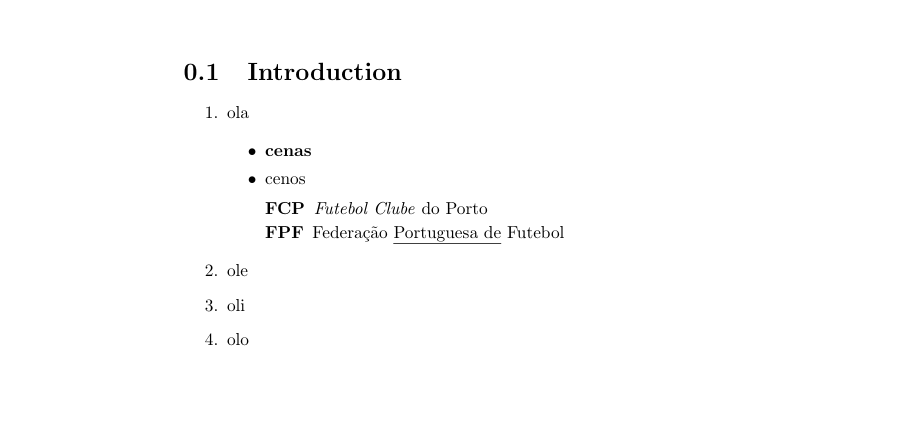
\includegraphics[width=\linewidth]{Exemplo1.png}
  \caption{Exemplo1}
  \label{Exemplo1}
\end{figure}



\subsubsection{Exemplo 2}

\paragraph{Texto Original}

\begin{verbatim}
\documentclass{report}
\usepackage[utf8]{inputenc}

\title{TestesPL}
\author{JoseJorgeGoncalo}
\date{May 2018}

\begin{document}

\maketitle

\section{Introduction}

*ola*
&ole&
_oli_

#O#

# ola
# ole
# oli
# olo

#N#

# cenas
# cenos

#FN#

#FO#

#D#

#[FCP] Futebol Clube do Porto
#[FPF] Federação Portuguesa de Futebol 

#FD#

$ Teste $

Vamos lá testar!

$$ Devia dar $

Será que vai dar?

$$$ TODOS juntos $

Todos juntos conseguimos.

#T#

>C

>L OlaCenas >FL

\begin{tabular}{\|c\|c\|c\|c\|}

\hline

A | B | C | D #
\hline
A | B | C | D #

\hline

\end{tabular}

#FT#

\end{document}

\end{verbatim}


\paragraph{Texto Produzido}

\begin{verbatim}
\documentclass{report}
\usepackage[utf8]{inputenc}

\title{TestesPL}
\author{JoseJorgeGoncalo}
\date{May 2018}

\begin{document}

\maketitle

\section{Introduction}

\textbf{ola}
\textit{ole}
\underline{oli}

\begin{enumerate}

\item ola
\item ole
\item oli
\item olo

\begin{itemize}

\item cenas
\item cenos

\end{itemize}

\end{enumerate}

\begin{description}

\item[FCP] Futebol Clube do Porto
\item[FPF] Federação Portuguesa de Futebol 

\end{description}

\chapter{ Teste }

Vamos lá testar!

\section{ Devia dar }

Será que vai dar?

\subsection{ TODOS juntos }

Todos juntos conseguimos.

\begin{table}

\centering

\caption{ OlaCenas }

\begin{tabular}{|c|c|c|c|}

\hline

A & B & C & D \\
\hline
A & B & C & D \\

\hline

\end{tabular}

\end{table}

\end{document}

\end{verbatim}

\paragraph{Resultado em formato PDF}

\paragraph{} De seguida apresentamos as imagens correspondentes ao texto acima descrito.

\begin{figure}[H]
  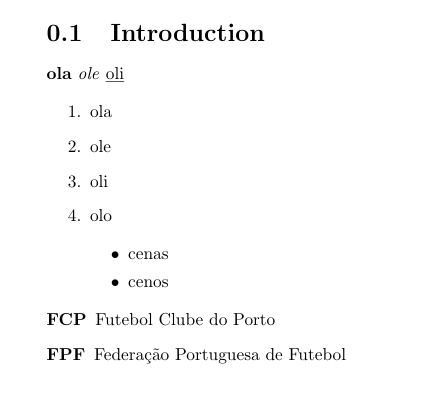
\includegraphics[width=\linewidth]{Exemplo2_1.png}
  \caption{exemplo2\_1}
  \label{exemplo2_1}
\end{figure}


\begin{figure}[H]
  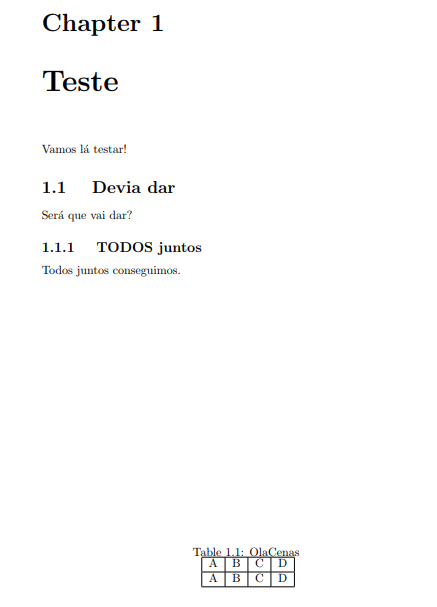
\includegraphics[width=\linewidth]{exemplo2_2.png}
  \caption{exemplo2\_2}
  \label{exemplo2_2}
\end{figure}


\subsubsection{Exemplo 3}

\paragraph{Texto Original}

\begin{verbatim}

\documentclass{report}
\usepackage[utf8]{inputenc}

\title{TestesPL}
\author{JoseJorgeGoncalo}
\date{May 2018}

\begin{document}

\maketitle

\section{Introduction}


#T#

>C

>L OlaCenas >FL

\begin{tabular}{\|c\|c\|c\|c\|}

\hline

*ola* | &ole& | C | D #
\hline
A | 

\begin{minipage}{1.5in}
#O#

# ola
# ole
# oli
# olo

#N#

# cenas
# cenos

#FN#

#FO# 
\end{minipage}
| _oli_ | D #

\hline

\end{tabular}

#FT#

\end{document}

\end{verbatim}


\paragraph{Texto Produzido}

\begin{verbatim}

\documentclass{report}
\usepackage[utf8]{inputenc}

\title{TestesPL}
\author{JoseJorgeGoncalo}
\date{May 2018}

\begin{document}

\maketitle

\section{Introduction}


\begin{table}

\centering

\caption{ OlaCenas }

\begin{tabular}{|c|c|c|c|}

\hline

\textbf{ola} & \textit{ole} & C & D \\
\hline
A & 

\begin{minipage}{1.5in}
\begin{enumerate}

\item ola
\item ole
\item oli
\item olo

\begin{itemize}

\item cenas
\item cenos

\end{itemize}

\end{enumerate} 
\end{minipage}
& \underline{oli} & D \\

\hline

\end{tabular}

\end{table}

\end{document}

\end{verbatim}

\paragraph{Resultado em formato PDF}

\paragraph{} De seguida apresentamos a imagem correspondente ao texto acima descrito.

\begin{figure}[H]
  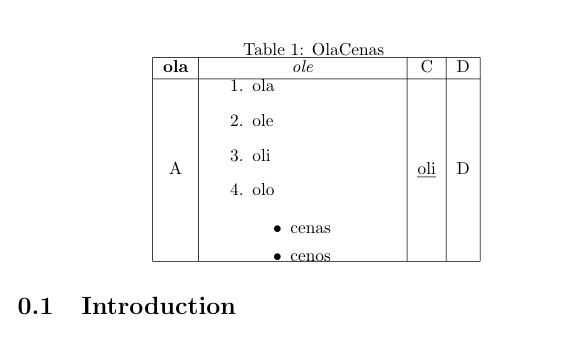
\includegraphics[width=\linewidth]{exemplo3.png}
  \caption{exemplo3}
  \label{exemplo3}
\end{figure}

\subsection{Código produzido}

\begin{verbatim}
%{
#include <stdio.h>
#include <stdlib.h>
#include <string.h>
#include <fcntl.h>
%}

%x LISTA NEGRITO ITALICO SUBLINHADO CABECALHO DICIONARIO ELEMENTO TABELA

%option stack

%%


#T# {
  printf("\\begin{table}");
  yy_push_state(TABELA);
}


<*>\\[*_&#$] {printf("%s",yytext);}

<CABECALHO>\$ {
  printf("}");
  int top = yy_top_state();

  //printf("TOP: %d\n",top);
  //if(top!=0){
    yy_pop_state();
  //}
  //else{ BEGIN 0; }
}

<NEGRITO>\* {
    printf("}");
    int top = yy_top_state();

    //printf("TOP: %d\n",top);
  //  if(top!=0){
      yy_pop_state();
  //  }
  //  else{ BEGIN 0; }
  }

<ITALICO>& {

    printf("}");

    int top = yy_top_state();

    //printf("TOP: %d\n",top);
  //  if(yy_top_state()!=0){
      yy_pop_state();
  //  }
  //  else{ BEGIN 0; }
}

<SUBLINHADO>_ {

    printf("}");

    int top = yy_top_state();

    //printf("TOP: %d\n",top);
  //  if(yy_top_state()!=0){
      yy_pop_state();
  //  }
  //  else{ BEGIN 0; }

}

<LISTA>#  {

    printf("\\item");
}

<LISTA>#FO# {
  printf("\\end{enumerate}");
  yy_pop_state();
}

<LISTA>#FN# {
  printf("\\end{itemize}");
  yy_pop_state();
}

<DICIONARIO>#\[[^#*_&]+\] {

    printf("\\item%s",yytext+1);
    
}

<DICIONARIO>#FD#  {
  printf("\\end{description}");
  yy_pop_state();
}

<TABELA>\\\> {printf(">");}

<TABELA>\>C {printf("\\centering");}

<TABELA>\>L {printf("\\caption{");}

<TABELA>\>FL {printf("}");}

<TABELA>\| {printf("&");}

<TABELA>\\\| {printf("|");}

<TABELA># {printf("\\\\");}

<TABELA>#FT# { printf("\\end{table}"); yy_pop_state();}

$+  {
  int tam = strlen(yytext);
  switch(tam){
    case 1: printf("\\chapter{"); break;
    case 2: printf("\\section{"); break;
    case 3: printf("\\subsection{"); break;
    default: printf("\\subsubsection{");
  }
  yy_push_state(CABECALHO);
}

<*>\* { 
    printf("\\textbf{");
    yy_push_state(NEGRITO);
 
    }

<*>&  { 
    printf("\\textit{");
    yy_push_state(ITALICO);


}

<*>_ { 

    printf("\\underline{");
    yy_push_state(SUBLINHADO);

}

<*>#O# { 
    printf("\\begin{enumerate}");
    yy_push_state(LISTA);
}

<*>#N# { 
    printf("\\begin{itemize}");
    yy_push_state(LISTA);
}

<*>#D# {
    printf("\\begin{description}");
    yy_push_state(DICIONARIO);
}


%%

int yywrap(){
  return 1;
}

int main(int argc, char** argv) {
  
  yylex();
  

  return 0;
}
\end{verbatim}


\section{Conclusão} \label{concl}

Em suma, podemos afirmar que o trabalho realizado foi concluído com sucesso. O nosso principal objetivo, conseguir realizar tudo o que era proposto no enunciado, foi conseguido, já que a nossa linguagem consegue abstrair o uso de “código latex” para os casos de o utilizador querer utilizar as marcas que estavam referidas no enunciado. Para além deste aspeto, ainda conseguimos implementar uns extras com o encadeamento das marcas (por exemplo uma mesma palavra pode ser escrita a itálico e sublinhada), uma linguagem simplista para o uso de tabelas e ainda escrevemos uma “main” que permitia ao utilizador colocar como input o nome dos ficheiros, desta forma é mais intuitiva trabalhar, do que efetuar um redireccionamento a partir da bash.

Não só conseguimos resolver o que era pedido e ainda acrescentamos uns extras, como também o núcleo da resolução do problema passa pelo uso de Expressões Regulares e também do \textit[flex}. O uso da \textit{stack} “nativa” do flex revelou-se uma ferramenta extremamente útil e eficaz, permitindo-nos, de uma forma mais fácil, aplicar então o encadeamento de instruções. Pelo facto mencionado anteriormente, podemos afirmar que conseguimos concluir o segundo objetivo delimitado conforme pretendido.

Mais uma vez, a realização deste projeto clarificou-nos o uso correto para a ferramenta \textit{flex} e o quão poderosa esta poderá ser aliada ainda a outras. Ficamos agradados com os resultados obtidos, e  verificamos que o uso de uma anotação do tipo \textit{Markdown} poderá facilitar, e muito, a produção de textos em latex, por exemplo.

\end{document}
